\documentclass[12pt]{article}
\usepackage{geometry}
\usepackage{url}
\usepackage{graphicx}
\usepackage{float}
\usepackage{pdflscape}
\usepackage{amsmath}
\title{\Huge Neural Networks \\
[6mm]
Assignment 4\\}
\author{Ravikiran Bhat\\
Rubanraj Ravichandran\\
Ramesh Kumar}

\begin{document}
\maketitle
\newpage
\newpage
\section{Mindmap}
 \begin{figure}[H]
    \centering
    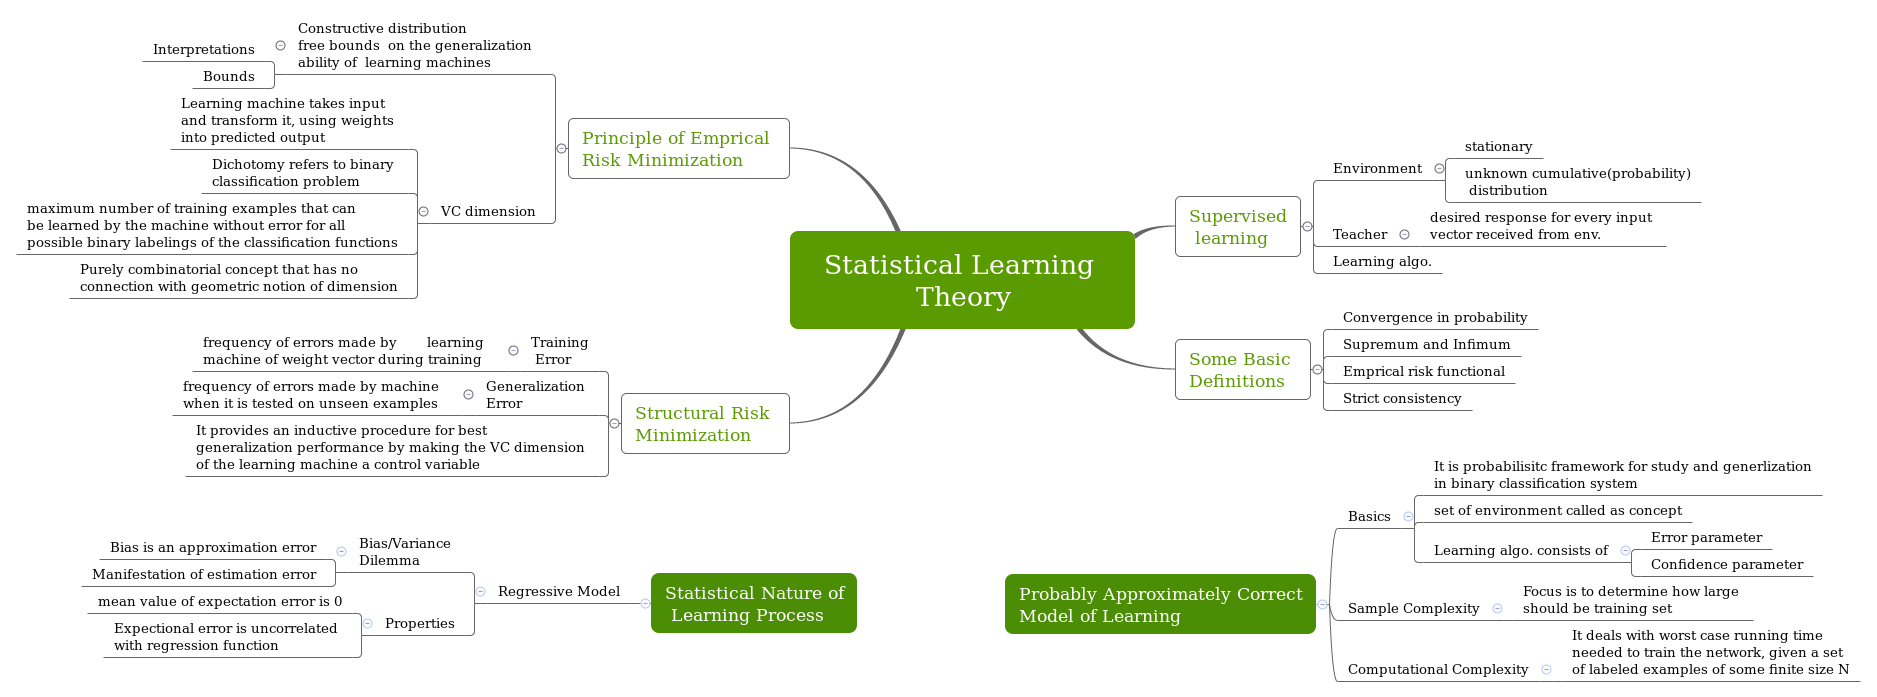
\includegraphics[scale=0.32,angle=90]{map.png}
  \end{figure}
\newpage 
\section{Exercise 2}
\begin{enumerate}
\item If the given set of rectangles Hr is axis aligned, then the VC(Hr) = 4. This is because, there exists at least one configuration of points (such as ${(1, 0),(0.1),(−1, 0),(0, −1)}$ ) that can be shattered. But a configuration of 5 points cannot be shattered by an axis alligned rectangle \cite{vcDimension}.
\item For the set of all circles Hc in the x,y plane, VC(Hc)=3 \cite{vcDimension}.
\item For the set Ht of all triangles in the x,y plan, the VC(Ht) = 7 \cite{vcDimension}.
\end{enumerate}

\section{Exercise 3 - Consistent learner}
 \begin{figure}[H]
	\centering
	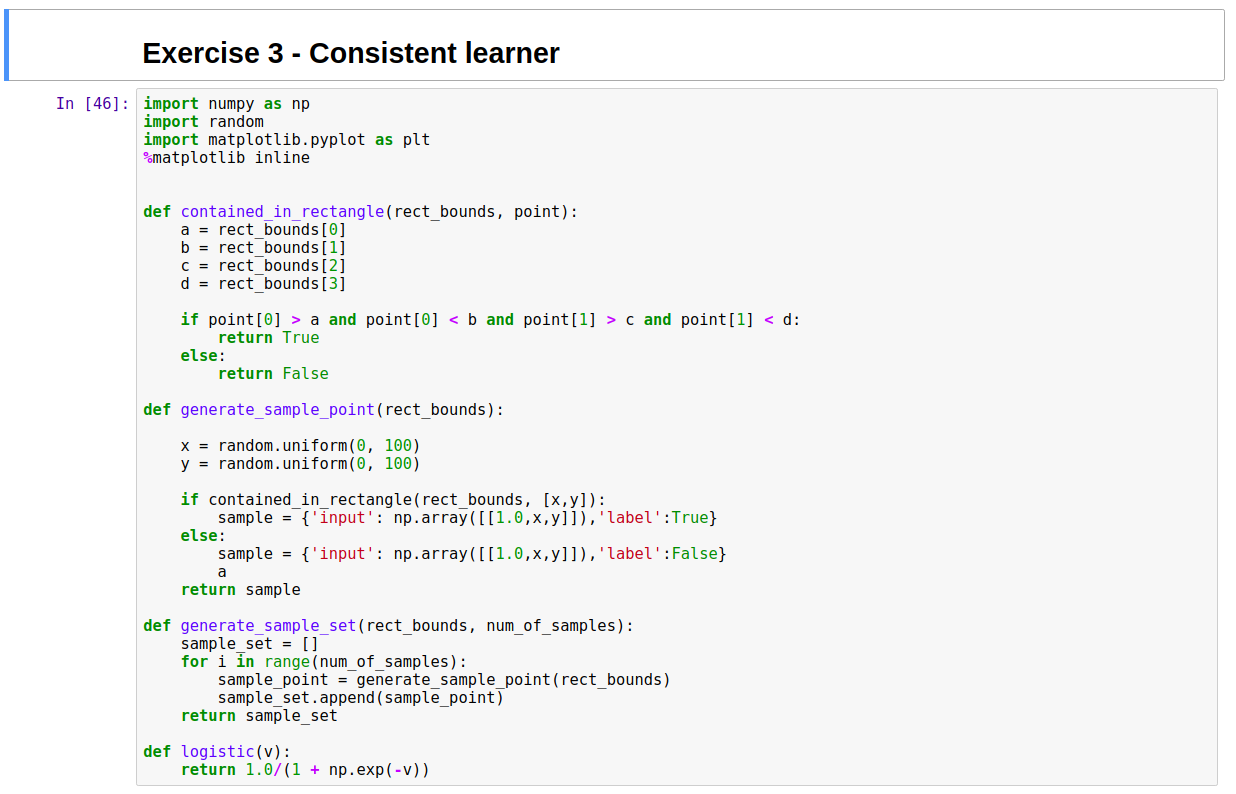
\includegraphics[scale=0.40]{ex3_1.png}
\end{figure}

 \begin{figure}[H]
	\centering
	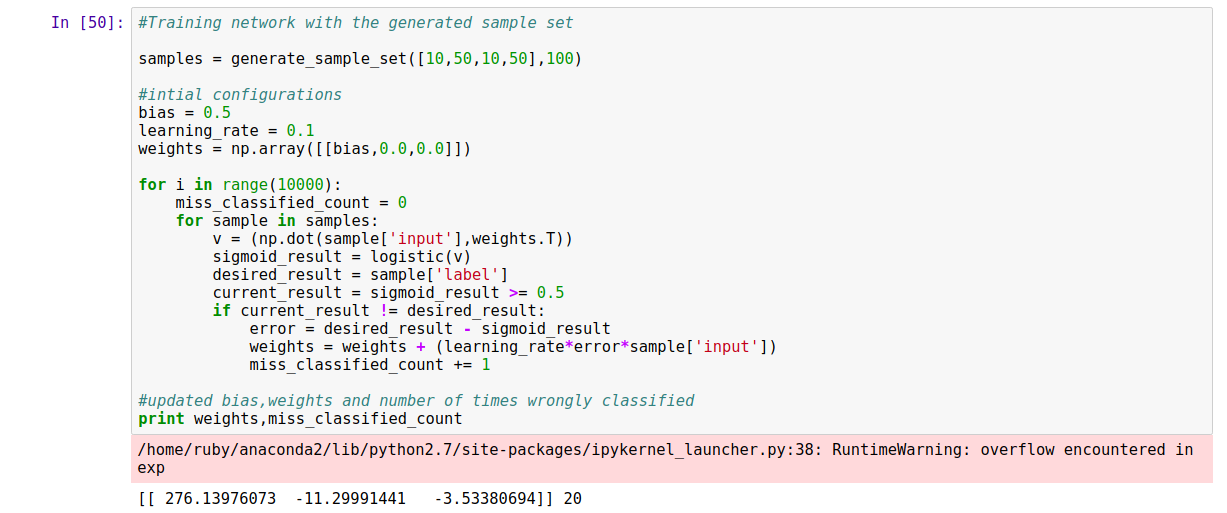
\includegraphics[scale=0.40]{ex3_2.png}
\end{figure}

 \begin{figure}[H]
	\centering
	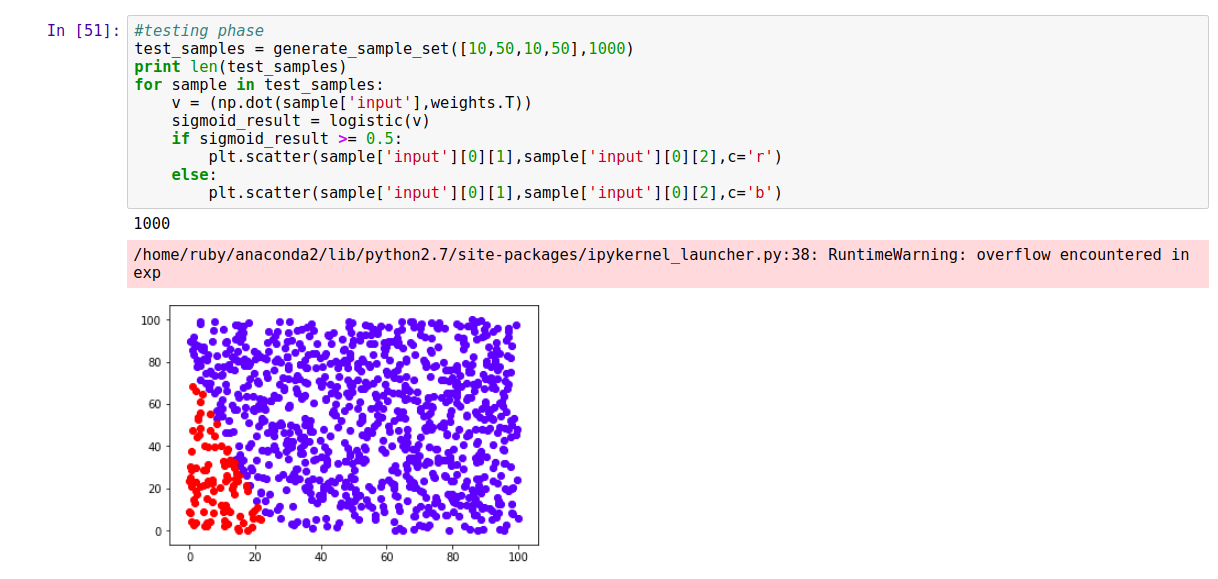
\includegraphics[scale=0.40]{ex3_3.png}
\end{figure}
\newpage
\bibliographystyle{plain}
\bibliography{bibtex}
\end{document}